\documentclass{standalone}
\usepackage{tikz}
\usetikzlibrary{patterns, positioning}

\begin{document}
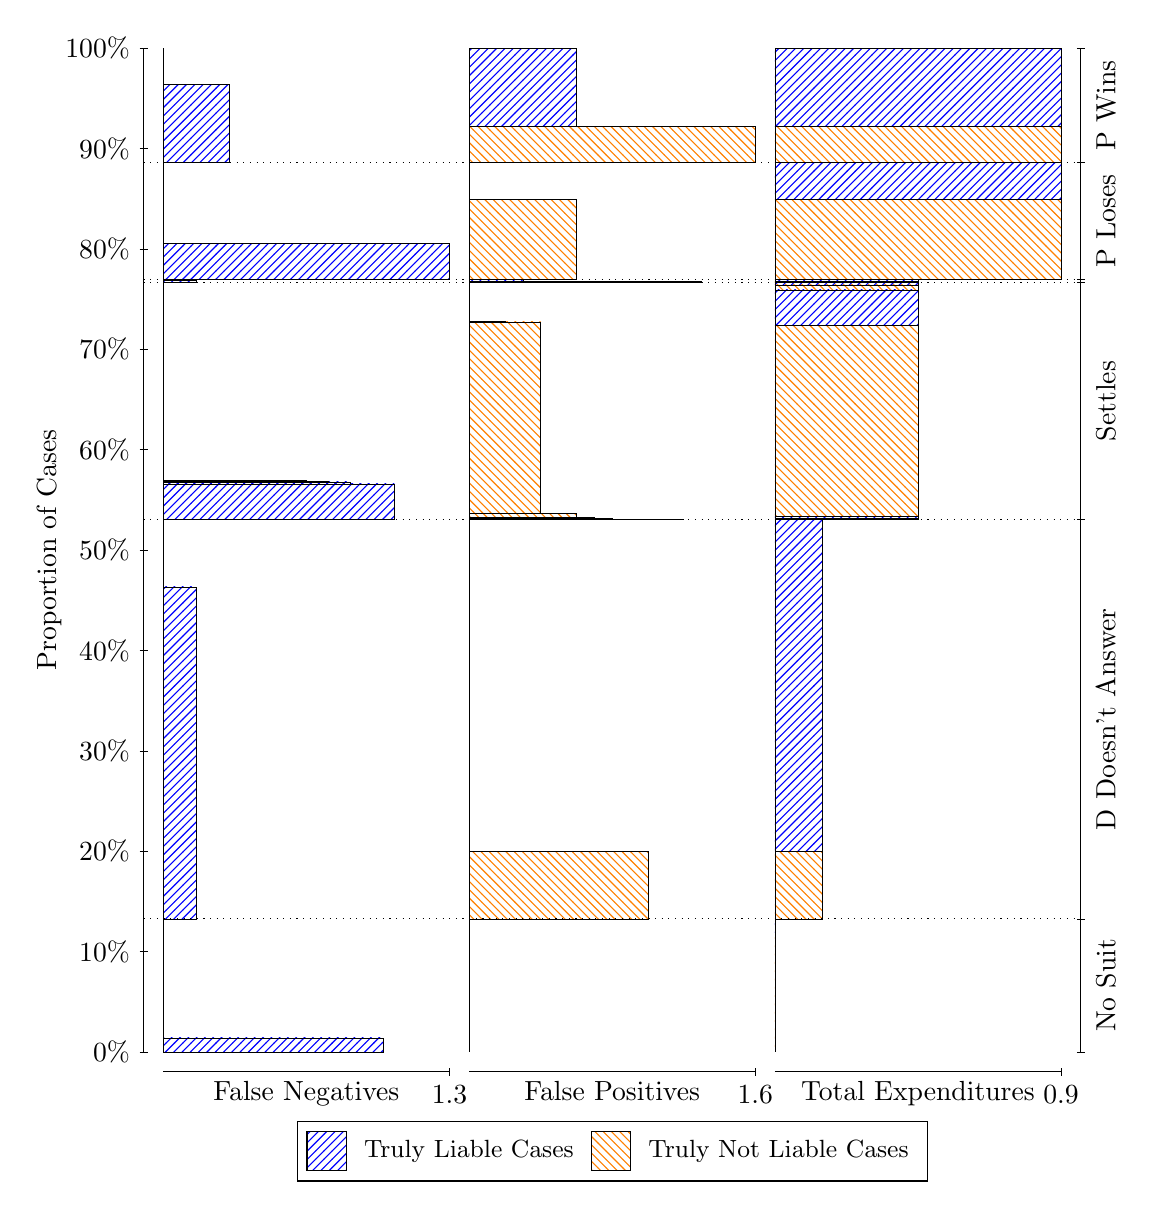
\begin{tikzpicture}
\draw[black, very thin] (1.5,1.75) -- (1.5,14.5);
\node[rotate=90, anchor=center] at (0.3, 8.125) {Proportion of Cases};
\draw[black, very thin] (1.45,1.75) -- (1.55,1.75);
\node[anchor=east] at (1.45, 1.75) {0\%};
\draw[black, very thin] (1.45,3.025) -- (1.55,3.025);
\node[anchor=east] at (1.45, 3.025) {10\%};
\draw[black, very thin] (1.45,4.3) -- (1.55,4.3);
\node[anchor=east] at (1.45, 4.3) {20\%};
\draw[black, very thin] (1.45,5.575) -- (1.55,5.575);
\node[anchor=east] at (1.45, 5.575) {30\%};
\draw[black, very thin] (1.45,6.85) -- (1.55,6.85);
\node[anchor=east] at (1.45, 6.85) {40\%};
\draw[black, very thin] (1.45,8.125) -- (1.55,8.125);
\node[anchor=east] at (1.45, 8.125) {50\%};
\draw[black, very thin] (1.45,9.4) -- (1.55,9.4);
\node[anchor=east] at (1.45, 9.4) {60\%};
\draw[black, very thin] (1.45,10.675) -- (1.55,10.675);
\node[anchor=east] at (1.45, 10.675) {70\%};
\draw[black, very thin] (1.45,11.95) -- (1.55,11.95);
\node[anchor=east] at (1.45, 11.95) {80\%};
\draw[black, very thin] (1.45,13.225) -- (1.55,13.225);
\node[anchor=east] at (1.45, 13.225) {90\%};
\draw[black, very thin] (1.45,14.5) -- (1.55,14.5);
\node[anchor=east] at (1.45, 14.5) {100\%};

\draw[black, very thin] (13.4,1.75) -- (13.4,14.5);
\draw[black, very thin] (13.35,1.75) -- (13.45,1.75);
\node[anchor=west] at (13.35, 1.75) {};
\draw[black, very thin] (13.35,3.4399) -- (13.45,3.4399);
\node[anchor=west] at (13.35, 3.4399) {};
\draw[black, very thin] (13.35,8.513) -- (13.45,8.513);
\node[anchor=west] at (13.35, 8.513) {};
\draw[black, very thin] (13.35,11.522) -- (13.45,11.522);
\node[anchor=west] at (13.35, 11.522) {};
\draw[black, very thin] (13.35,11.557) -- (13.45,11.557);
\node[anchor=west] at (13.35, 11.557) {};
\draw[black, very thin] (13.35,13.043) -- (13.45,13.043);
\node[anchor=west] at (13.35, 13.043) {};
\draw[black, very thin] (13.35,14.5) -- (13.45,14.5);
\node[anchor=west] at (13.35, 14.5) {};

\draw[black, very thin, pattern color=blue, pattern=north east lines] (1.75,1.75) rectangle (4.5449,1.9278);
\draw[black, very thin, pattern color=orange, pattern=north west lines] (1.75,1.9278) rectangle (1.75,3.4399);
\draw[black, very thin, pattern color=blue, pattern=north east lines] (1.75,3.4399) rectangle (2.1692,7.6572);
\draw[black, very thin, pattern color=orange, pattern=north west lines] (1.75,7.6572) rectangle (1.75,8.513);
\draw[black, very thin, pattern color=blue, pattern=north east lines] (1.75,8.513) rectangle (4.6846,8.9657);
\draw[black, very thin, pattern color=blue, pattern=north east lines] (1.75,8.9657) rectangle (4.4051,8.966);
\draw[black, very thin, pattern color=blue, pattern=north east lines] (1.75,8.966) rectangle (4.1256,8.9891);
\draw[black, very thin, pattern color=blue, pattern=north east lines] (1.75,8.9891) rectangle (3.8462,8.9929);
\draw[black, very thin, pattern color=blue, pattern=north east lines] (1.75,8.9929) rectangle (3.5667,9.0078);
\draw[black, very thin, pattern color=blue, pattern=north east lines] (1.75,9.0078) rectangle (3.2872,9.0089);
\draw[black, very thin, pattern color=blue, pattern=north east lines] (1.75,9.0089) rectangle (3.0077,9.0113);
\draw[black, very thin, pattern color=blue, pattern=north east lines] (1.75,9.0113) rectangle (2.7282,9.0117);
\draw[black, very thin, pattern color=blue, pattern=north east lines] (1.75,9.0117) rectangle (2.4487,9.0127);
\draw[black, very thin, pattern color=orange, pattern=north west lines] (1.75,9.0127) rectangle (1.75,11.522);
\draw[black, very thin, pattern color=blue, pattern=north east lines] (1.75,11.522) rectangle (2.1692,11.545);
\draw[black, very thin, pattern color=orange, pattern=north west lines] (1.75,11.545) rectangle (1.75,11.557);
\draw[black, very thin, pattern color=blue, pattern=north east lines] (1.75,11.557) rectangle (5.3833,12.022);
\draw[black, very thin, pattern color=orange, pattern=north west lines] (1.75,12.022) rectangle (1.75,13.043);
\draw[black, very thin, pattern color=blue, pattern=north east lines] (1.75,13.043) rectangle (2.5885,14.035);
\draw[black, very thin, pattern color=orange, pattern=north west lines] (1.75,14.035) rectangle (1.75,14.5);
\draw[black, very thin, pattern color=orange, pattern=north west lines] (5.6333,1.75) rectangle (5.6333,3.2621);
\draw[black, very thin, pattern color=blue, pattern=north east lines] (5.6333,3.2621) rectangle (5.6333,3.4399);
\draw[black, very thin, pattern color=orange, pattern=north west lines] (5.6333,3.4399) rectangle (7.9042,4.2957);
\draw[black, very thin, pattern color=blue, pattern=north east lines] (5.6333,4.2957) rectangle (5.6333,8.513);
\draw[black, very thin, pattern color=orange, pattern=north west lines] (5.6333,8.513) rectangle (8.3583,8.5135);
\draw[black, very thin, pattern color=orange, pattern=north west lines] (5.6333,8.5135) rectangle (8.1313,8.5137);
\draw[black, very thin, pattern color=orange, pattern=north west lines] (5.6333,8.5137) rectangle (7.9042,8.5153);
\draw[black, very thin, pattern color=orange, pattern=north west lines] (5.6333,8.5153) rectangle (7.6771,8.5164);
\draw[black, very thin, pattern color=orange, pattern=north west lines] (5.6333,8.5164) rectangle (7.45,8.531);
\draw[black, very thin, pattern color=orange, pattern=north west lines] (5.6333,8.531) rectangle (7.2229,8.5362);
\draw[black, very thin, pattern color=orange, pattern=north west lines] (5.6333,8.5362) rectangle (6.9958,8.5923);
\draw[black, very thin, pattern color=orange, pattern=north west lines] (5.6333,8.5923) rectangle (6.7687,8.5931);
\draw[black, very thin, pattern color=orange, pattern=north west lines] (5.6333,8.5931) rectangle (6.5417,11.023);
\draw[black, very thin, pattern color=blue, pattern=north east lines] (5.6333,11.023) rectangle (6.0875,11.024);
\draw[black, very thin, pattern color=blue, pattern=north east lines] (5.6333,11.024) rectangle (5.8604,11.024);
\draw[black, very thin, pattern color=blue, pattern=north east lines] (5.6333,11.024) rectangle (5.6333,11.522);
\draw[black, very thin, pattern color=orange, pattern=north west lines] (5.6333,11.522) rectangle (8.5854,11.534);
\draw[black, very thin, pattern color=blue, pattern=north east lines] (5.6333,11.534) rectangle (6.3146,11.557);
\draw[black, very thin, pattern color=orange, pattern=north west lines] (5.6333,11.557) rectangle (6.9958,12.578);
\draw[black, very thin, pattern color=blue, pattern=north east lines] (5.6333,12.578) rectangle (5.6333,13.043);
\draw[black, very thin, pattern color=orange, pattern=north west lines] (5.6333,13.043) rectangle (9.2667,13.508);
\draw[black, very thin, pattern color=blue, pattern=north east lines] (5.6333,13.508) rectangle (6.9958,14.5);
\draw[black, very thin, pattern color=orange, pattern=north west lines] (9.5167,1.75) rectangle (9.5167,3.2621);
\draw[black, very thin, pattern color=blue, pattern=north east lines] (9.5167,3.2621) rectangle (9.5167,3.4399);
\draw[black, very thin, pattern color=orange, pattern=north west lines] (9.5167,3.4399) rectangle (10.122,4.2957);
\draw[black, very thin, pattern color=blue, pattern=north east lines] (9.5167,4.2957) rectangle (10.122,8.513);
\draw[black, very thin, pattern color=orange, pattern=north west lines] (9.5167,8.513) rectangle (11.333,8.5295);
\draw[black, very thin, pattern color=blue, pattern=north east lines] (9.5167,8.5295) rectangle (11.333,8.5472);
\draw[black, very thin, pattern color=orange, pattern=north west lines] (9.5167,8.5472) rectangle (11.333,10.977);
\draw[black, very thin, pattern color=blue, pattern=north east lines] (9.5167,10.977) rectangle (11.333,11.429);
\draw[black, very thin, pattern color=orange, pattern=north west lines] (9.5167,11.429) rectangle (11.333,11.493);
\draw[black, very thin, pattern color=blue, pattern=north east lines] (9.5167,11.493) rectangle (11.333,11.522);
\draw[black, very thin, pattern color=orange, pattern=north west lines] (9.5167,11.522) rectangle (11.333,11.534);
\draw[black, very thin, pattern color=blue, pattern=north east lines] (9.5167,11.534) rectangle (11.333,11.557);
\draw[black, very thin, pattern color=orange, pattern=north west lines] (9.5167,11.557) rectangle (13.15,12.578);
\draw[black, very thin, pattern color=blue, pattern=north east lines] (9.5167,12.578) rectangle (13.15,13.043);
\draw[black, very thin, pattern color=orange, pattern=north west lines] (9.5167,13.043) rectangle (13.15,13.508);
\draw[black, very thin, pattern color=blue, pattern=north east lines] (9.5167,13.508) rectangle (13.15,14.5);
\draw[black, dotted] (1.5,3.4399) -- (13.4,3.4399);
\draw[black, dotted] (1.5,8.513) -- (13.4,8.513);
\draw[black, dotted] (1.5,11.522) -- (13.4,11.522);
\draw[black, dotted] (1.5,11.557) -- (13.4,11.557);
\draw[black, dotted] (1.5,13.043) -- (13.4,13.043);
\draw[black, very thin] (1.75,1.5) -- (5.3833,1.5);
\node[anchor=north] at (3.5667, 1.5) {False Negatives};
\draw[black, very thin] (5.3833,1.45) -- (5.3833,1.55);
\node[anchor=north] at (5.3833, 1.45) {1.3};

\draw[black, very thin] (5.6333,1.5) -- (9.2667,1.5);
\node[anchor=north] at (7.45, 1.5) {False Positives};
\draw[black, very thin] (9.2667,1.45) -- (9.2667,1.55);
\node[anchor=north] at (9.2667, 1.45) {1.6};

\draw[black, very thin] (9.5167,1.5) -- (13.15,1.5);
\node[anchor=north] at (11.333, 1.5) {Total Expenditures};
\draw[black, very thin] (13.15,1.45) -- (13.15,1.55);
\node[anchor=north] at (13.15, 1.45) {0.9};

\node[black, centered, rotate=90] at (13.72, 2.5949) {No Suit};
\node[black, centered, rotate=90] at (13.72, 5.9764) {D Doesn't Answer};
\node[black, centered, rotate=90] at (13.72, 10.018) {Settles};

\node[black, centered, rotate=90] at (13.72, 12.3) {P Loses};
\node[black, centered, rotate=90] at (13.72, 13.772) {P Wins};

\draw (7.449999999999999,1.5) node[draw=none] (baseCoordinate) {};
\begin{scope}[align=center]
        \matrix[scale=0.5, draw=black, below=0.5cm of baseCoordinate, nodes={draw}, column sep=0.1cm]{
            \node[rectangle, draw, minimum width=0.5cm, minimum height=0.5cm, pattern=north east lines, pattern color=blue] {}; &
            \node[draw=none, font=\small] (B) {Truly Liable Cases}; &
            \node[rectangle, draw, minimum width=0.5cm, minimum height=0.5cm, pattern=north west lines, pattern color=orange] {}; &
            \node[draw=none, font=\small] (B) {Truly Not Liable Cases}; \\
            };
\end{scope}

\end{tikzpicture}
\end{document}